Die Nacht im belegten 8~Mann Zimmer war in Ordnung, zumindest für mich.
Der Christian hat mit dem ersten Wort über seine Rückenschmerzen geklagt, was für ein Lappen.
Nachdem ich meinte, dass sich kaum einer gesund gelegen hat und er sich einfach bewegen soll, sank das Gejammer auf ein erträgliches Maß.
Das Frühstück war essbar und dann ging es zur Stadtführung.
Mit dem Linienbus ging es auf dem \FOREIGN{Interstate} für 30~Minuten Richtung \FOREIGN{Downtown}\footnote{Innenstadt}.
Dort angekommen führte uns unser obdachloser Stadtführer zur Stadtbibliothek, in ein Hotel, weil bei diesem die Aufzüge außen angebracht sind und man so die nähere Umgebung überblicken kann, in ein Büchergeschäft mit Künstlerateliers und zu einem Coffeeshop für einen kurzen Stopp.
Danach ging es weiter zum ehemaligen Bauernmarkt, der heute eine reine Fastfoodhalle ist, zur Disney Oper, nach \FOREIGN{Little Tokyo} und noch in ein mexikanisches Viertel.
Dort endete die anstrengende Rennerei.

Mit unseren neuen Bekanntschaften den Franzosen Maximili\textbf{e}n Ortiz und Pierre Bour (sie sind anschließend nach \TOWN{San Diego} weiter, um von dort den \FOREIGN{Pacific Crest Trail} zu laufen, was sie auch geschafft haben!), dem käsebleichen Hayden aus Manchester,

\begin{tikzpicture}[remember picture, overlay]
\node[inner sep=0pt, yshift=-.2\paperheight] at (current page.north) {%
	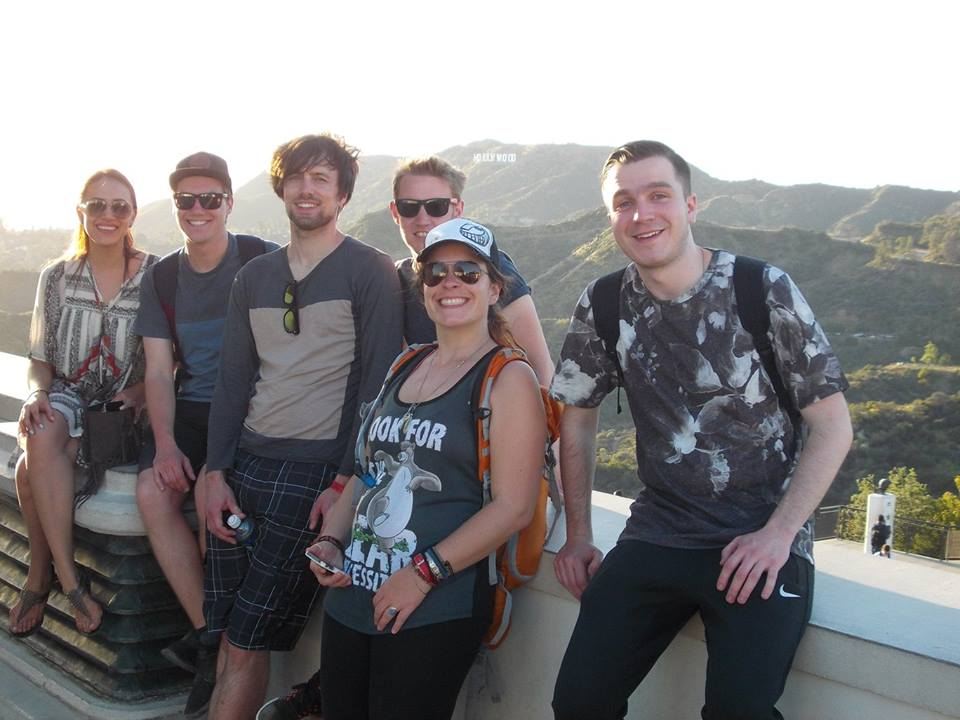
\includegraphics[width=\paperwidth,height=.5\paperheight]{16/la_gang.jpg};%
};
%\node[inner sep=0pt, yshift=.25\paperheight] at (current page.south) {%
%	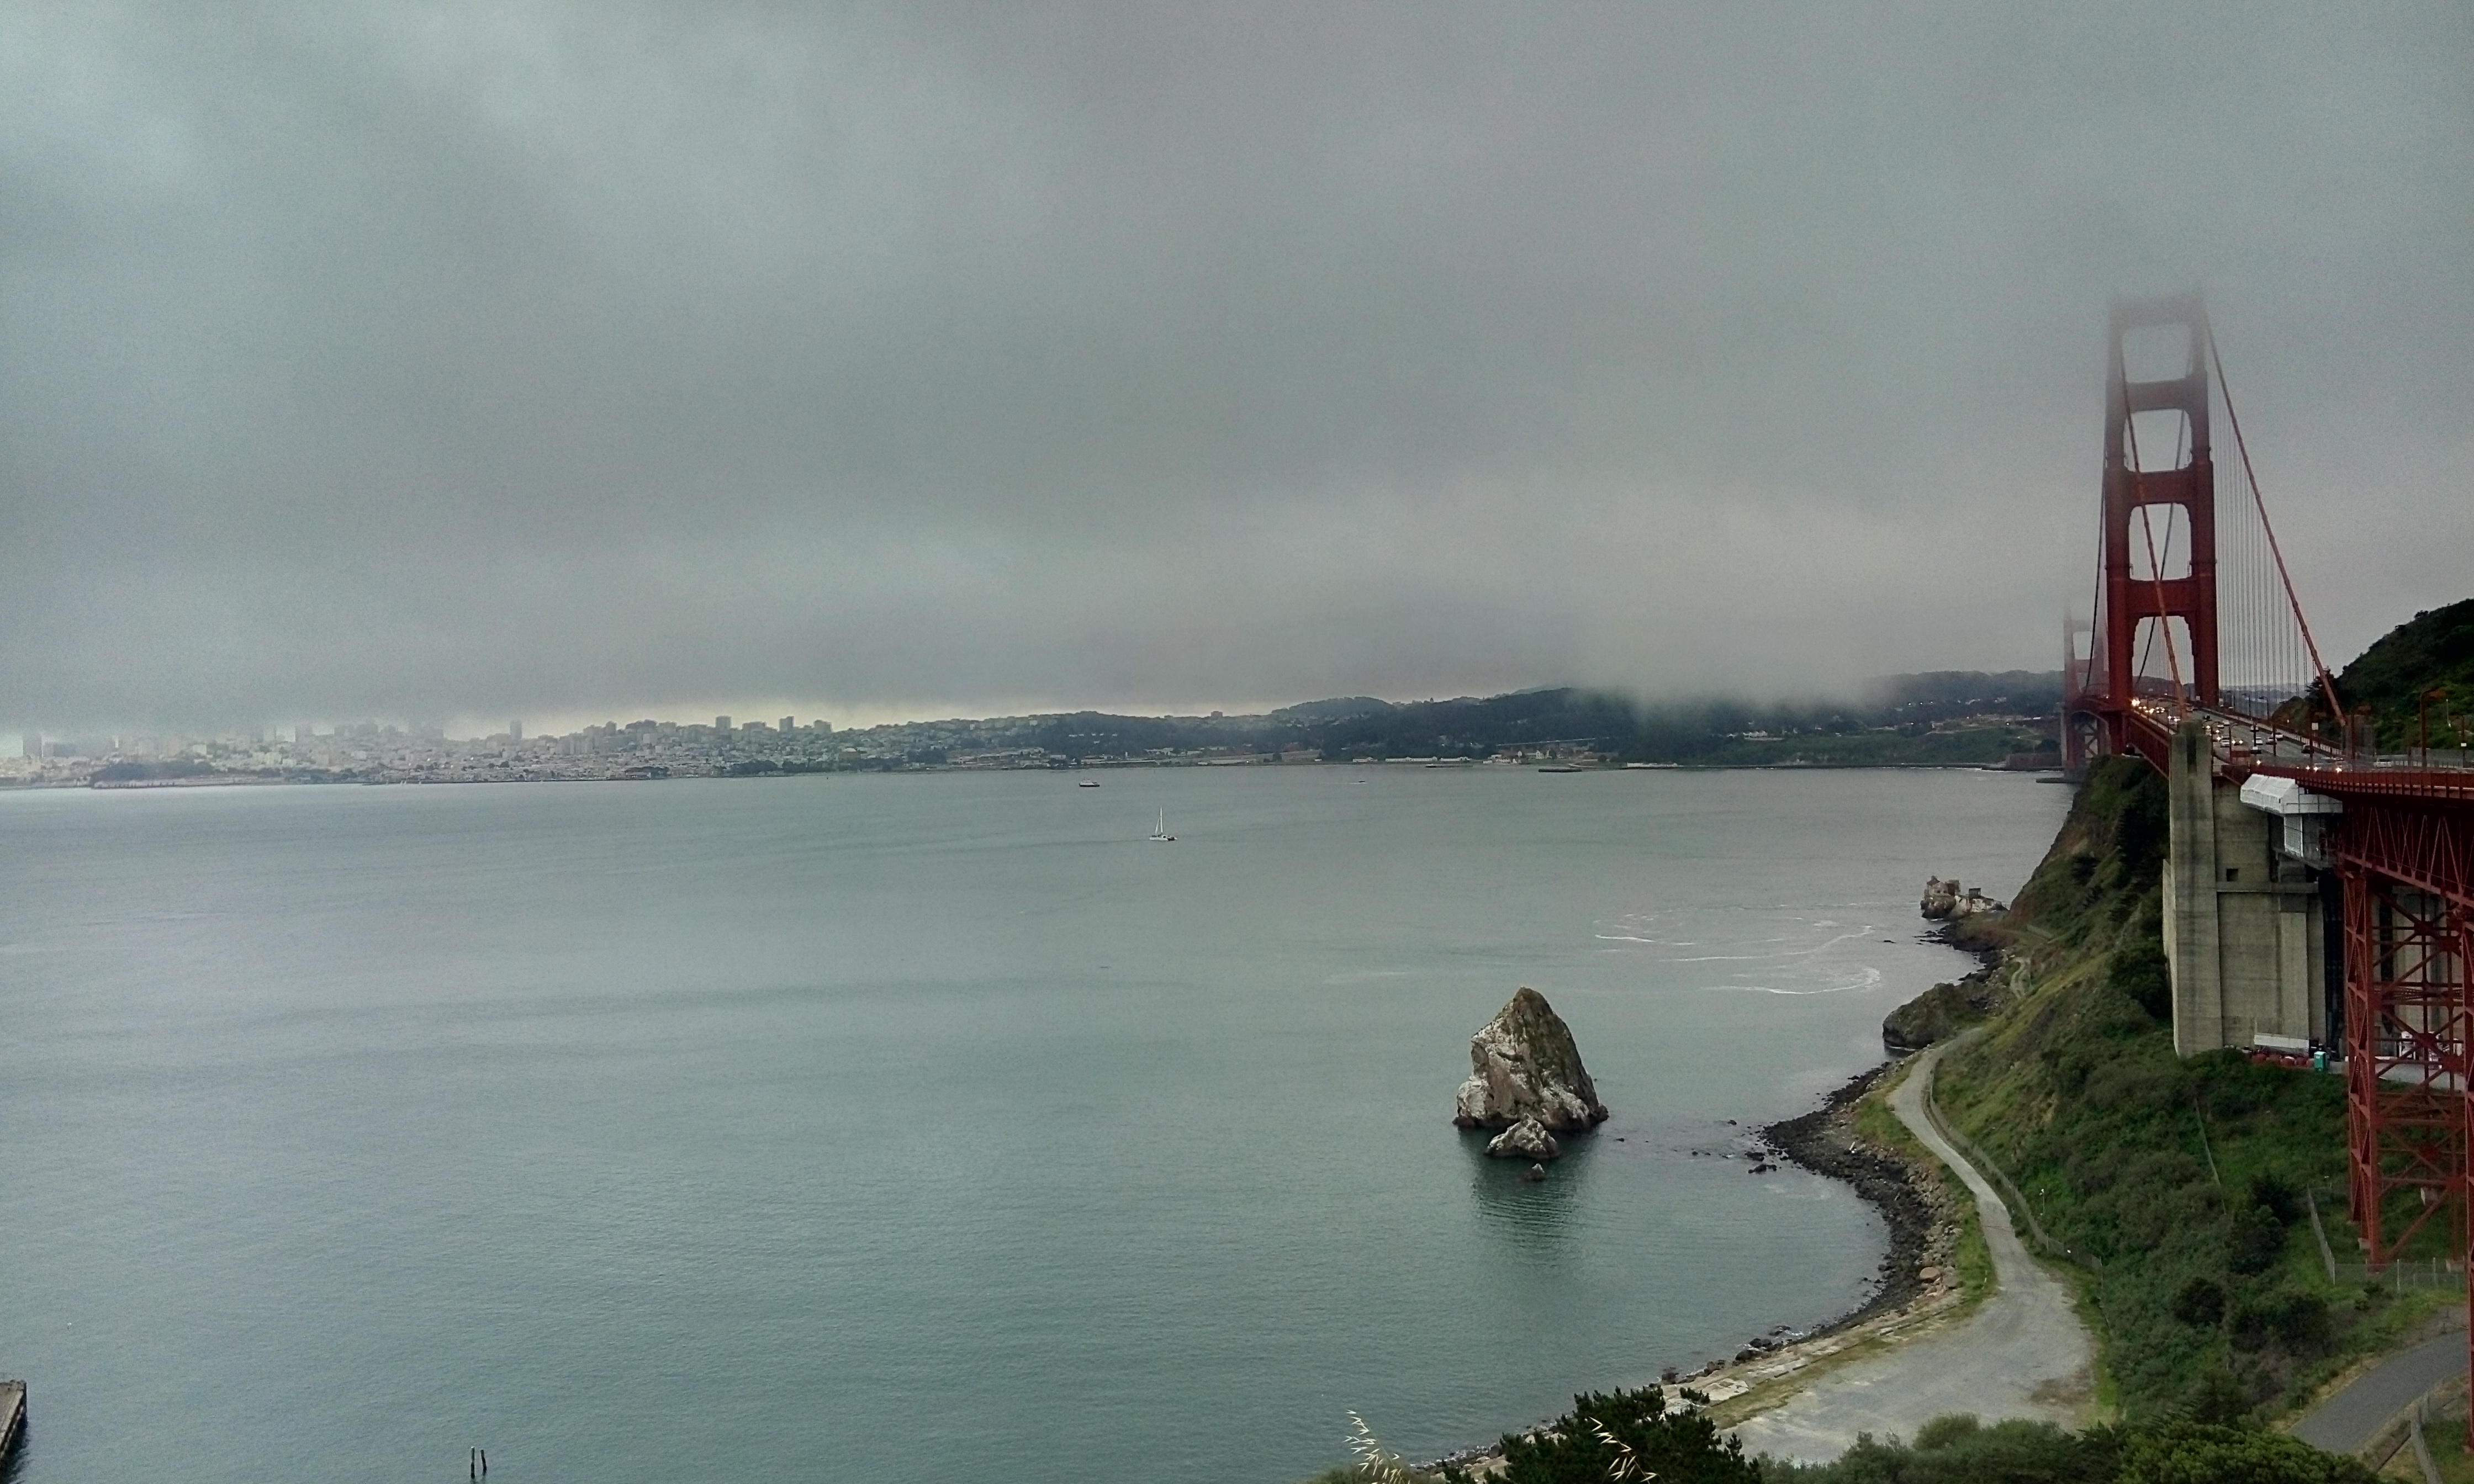
\includegraphics[width=\paperwidth,height=.5\paperheight]{21/image20160420_193101911.jpg};%
%};
\end{tikzpicture}

\vspace*{.3\paperheight}

\noindent
Manchester, der Weltreisenden Schweizerin Oona Baumier und der mexikanischen Mexikanerin Natalia Lopez ging es mit einer Uber-Fahrt zum Griffith \FOREIGN{Observatory}\footnote{Sternwarte}.
Zumindest in die Nähe.
Denn bis hoch ließen wir uns nicht fahren, das hätte 40~Minuten Stop\&Go bedeutet und wir gingen stattdessen zu Fuß.
Hayden wurde beim Aufstieg nochmals bleicher, weil er es nicht so mit engen, abschüssigen Trampelpfaden hat.
Mit Händchen halten haben wir ihn dann trotzdem hoch bekommen.
Das \FOREIGN{Observatory} hatten wir zwar knapp verfehlt, aber der angelaufene Hügel dahinter bot eh die bessere Aussicht.
Von dort aus hatte man auch eine gute Aussicht auf den berühmten Hollywood Schriftzug.

Von dort stiegen wir zum \FOREIGN{Observatory} ab, was wieder ein gewisses Drama bedeutete.
Wer was für unser Sonnensystem übrig hat, ist dort ganz gut aufgehoben.
Ich fand nur die Waagen zum Anzeigen des eigenen Gewichts (in lbs, also Pfund) auf dem jeweiligen Planeten ganz interessant.
Im Anschluss stand der richtige Abstieg an.
Da der Aufstieg in rund 20~Minuten möglich war, erwarteten wir eine ähnliche Zeit\dots es wurde allerdings eine gute Stunde.
Unten angekommen, dachten wir nochmal kurz über eine Uber-Fahrt nach, bis zur nächsten Bushaltestelle war es aber auch nicht weit.
Dort angekommen hatte sich der Uber-Preis bereits verdoppelt.
Ob es an der Anzahl verfügbarer Fahrer, der fortgeschrittenen Uhrzeit (es dämmerte bereits) oder der Gegend lag, lässt sich nur mutmaßen.
Der Bus kam dann und nach 50~Minuten waren wir am Hostel.

Von dort ging es mit nüchternem Magen zum nahegelegenen Pub \FOREIGN{``Ye Olde Kings Head''} auf ein paar Runden Bier.
Nach Runde drei verging mir der Durst, aber der Christian war auch nach Runde fünf derart unterhopft, dass er sich eines herrenlosen Bieres annahm.
Gegen 2~Uhr hat der Pub alle Gäste vor die Tür gesetzt und wir gingen heim, wovon Christian nichts mehr weiß\dots\\[1em]

\marginline{\texttt{Gegen\-dar\-stellung}}
\fbox{%
\parbox{.9\textwidth}{%
Es war kein \glqq herrenloses Bier\grqq\, sondern Thorstens.
Denn der war währenddessen sehr intensiv mit der Mexikanerin beschäftigt und konnte sich diesem nicht widmen.}
}
